\documentclass[10pt,a4paper]{article}

% Packages - Optimized margins to give more text area
\usepackage[margin=1.5cm, top=1.5cm, bottom=1.5cm]{geometry}
\usepackage{graphicx}
\usepackage{url}
\usepackage{float}
\usepackage{caption}

% Tightened spacing to pull content upwards
\setlength{\parindent}{0pt}
\setlength{\parskip}{3pt}
\captionsetup{font=small, labelfont=bf, skip=3pt}

% Suppress extra space around section headers
\usepackage{titlesec}
\titlespacing*{\section}{0pt}{8pt plus 2pt minus 2pt}{3pt plus 1pt}

% Title layout optimizations
\title{\vspace{-2cm}\bfseries\Large Analysis of Reported Measles Cases in Five European Countries (2015--2024)}
\author{Janneke de Haart}
\date{Period 1: 2026}

\begin{document}

\maketitle
\vspace{-1.1cm}

\section{Introduction}
Measles is a contagious disease that can be prevented by vaccination. By analyzing previously reported cases it is possible to observe the changes in case numbers over time and how they differ between countries. 
The purpose of this project is to answer the research question: Which selected European country had the highest number of reported measles cases between 2015 and 2024, and how did the case numbers change over this period?

\section{Dataset}
The Dataset used for this project was obtained from Our World in Data and it contains reported measles cases by country and year.
Five European countries were selected: the Netherlands, Belgium, Germany, France and Italy.
The variables used for the project were Country, Years and the number of reported measles cases.

\section{Methods}
The analysis was performed using the R programming language and Visual Studio Code.
First, the dataset was imported using \texttt{read.csv()} and inspected using \texttt{head()}, \texttt{str()}, and \texttt{summary()}. The column containing reported measles cases was renamed to \texttt{Measles\_cases}. Afterwards, the data was filtered to the five selected European countries and the years 2015 to 2024. The \texttt{aggregate()} function was used to calculate the highest total and the highest yearly peak for each of the selected countries. Lastly two plots were created using base R: a line plot showing the yearly annual reported cases and a bar plot showing the total number of reported cases in the chosen time period.

\section{Results}
Italy had the highest number of reported cases, with 9,722 cases between 2015 and 2024. France was second with 6,701 reported cases. Germany with 5,601, Belgium with 1,666 and the Netherlands with 354 reported cases.
Italy also had the highest yearly peak, with 4,042 reported cases in the year 2017. France reached its peak in 2018 with 2,921 reported cases, while Germany reached 2,464 cases in 2015. Belgium and the Netherlands both reached their highest yearly peak in 2024, with Belgium reaching 526 cases and the Netherlands reaching 202 reported cases.
The number of reported cases varied considerably between years and countries.

% First plot: Annual cases - scaled slightly down to fit easily
\begin{figure}[H]
    \centering
    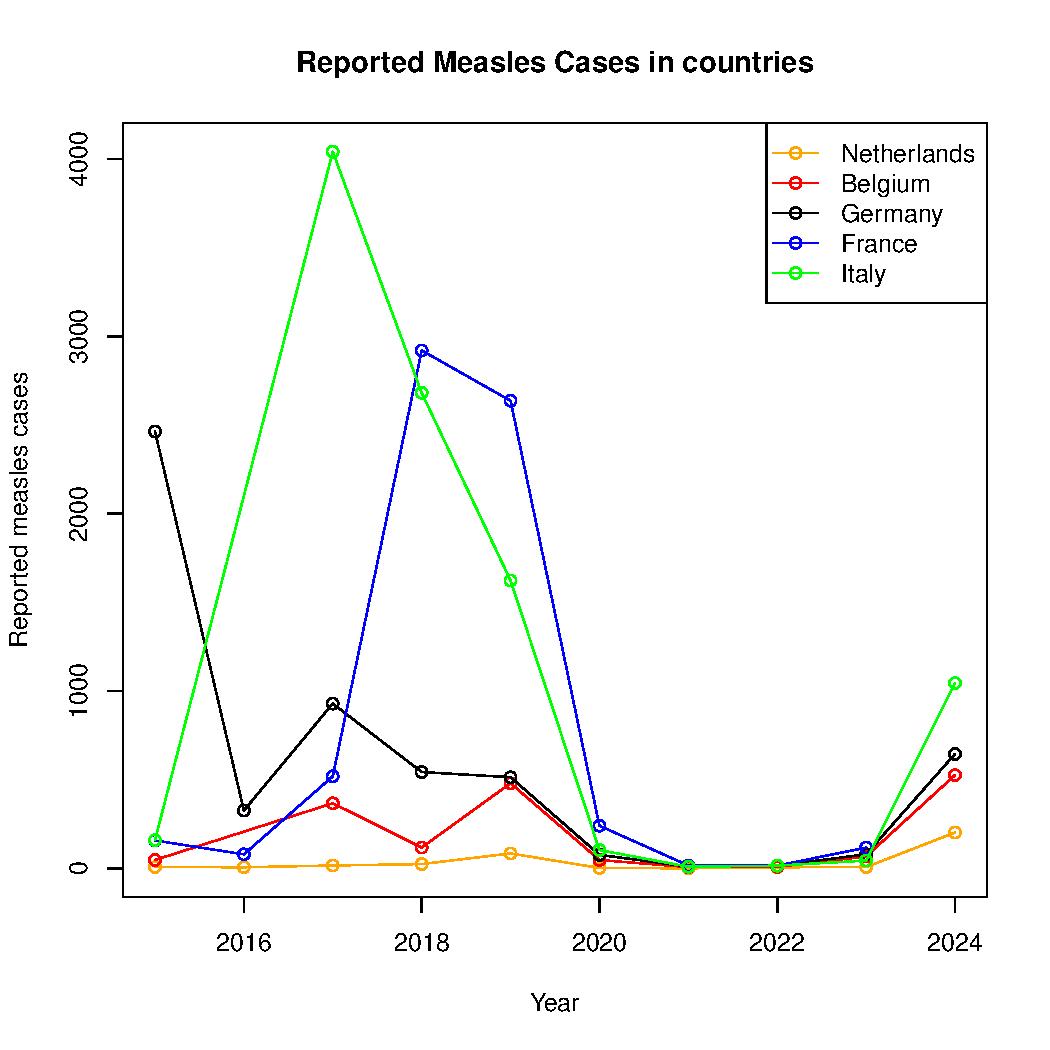
\includegraphics[width=0.52\textwidth]{Rplots_page_1.pdf}
    \vspace{-4pt}
    \caption{Annual reported measles cases in five European countries, 2015--2024.}
    \label{fig:annual}
\end{figure}

Figure~\ref{fig:total} compares the total reported cases for each country. Italy had the highest total with 9,722 cases, followed by France with 6,701 and Germany with 5,601. Belgium recorded 1,666 cases, while the Netherlands recorded 354 cases.

% Second plot: Total cases - scaled slightly down to fit easily
\begin{figure}[H]
    \centering
    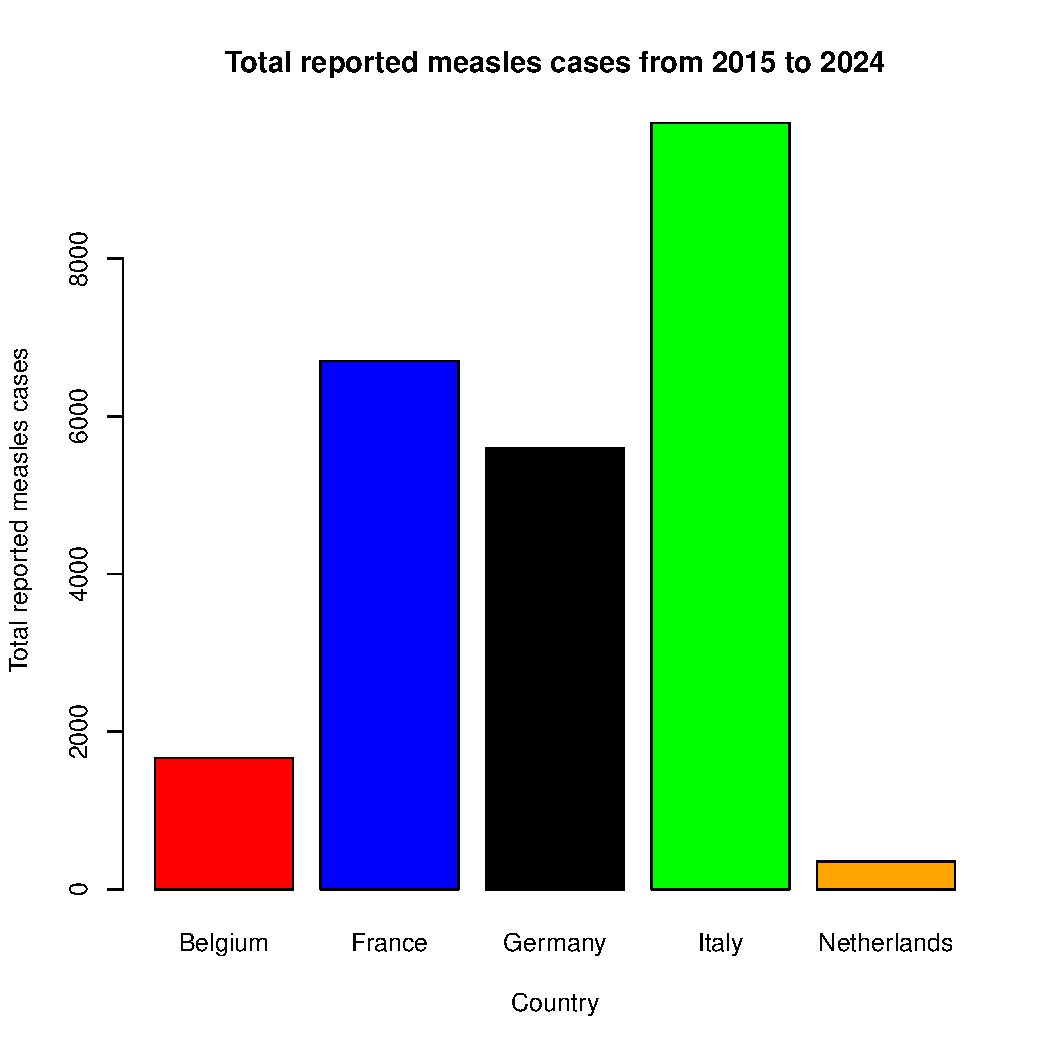
\includegraphics[width=0.52\textwidth]{Rplots_page_2.pdf}
    \vspace{-4pt}
    \caption{Total reported measles cases by country between 2015 and 2024.}
    \label{fig:total}
\end{figure}

\section{Conclusion}
Among the five selected European countries Italy had the highest total number of reported measles cases between 2015 and 2024, with 9,722 cases.
The obtained results show considerable differences between years and countries, including a period of low reported case numbers between 2020 and 2022.

\section*{Reference}
\small % Sizing down reference block slightly to ensure it stays on page 2
Our World in Data. (2026). \textit{Reported cases of measles}.\\
\url{https://ourworldindata.org}

\end{document}
